\section{Etapa 1}
\subsection{Selección de caso de uso}
Uno de los principales problemas de hacer ingeniería de rendimiento para software en la nube es que no existen aplicaciones de referencia que hayan ganado popularidad o cuyo desarrollo se encuentre activo. A pesar de esto y de su reciente adopción, la industria ha empezado a reconocer casos de uso en donde las aplicaciones \emph{serverless} encajan mejor. Amazon Web Services(AWS)\cite{serverless-architecture-patterns} reconoce cinco patrones de uso predominantes en su servicio AWS Lambda:
\begin{enumerate}
    \item Procesamiento de datos dirigidos por eventos.
    \item Aplicaciones Web.
    \item Aplicaciones móviles e Internet las cosas (IoT).
    \item Ecosistemas de aplicaciones \emph{serverless}.
    \item Flujos de trabajo dirigidos por eventos.
\end{enumerate}
 
Uno de las aplicaciones más comunes en \emph{serverless} es desencadenar acciones luego de que ocurre un evento (1), por ejemplo luego de la modificación de un registro en una base de datos o bien luego de que se publica un mensaje en una cola de mensajería. Esto puede provocar que se active una función Lambda\footnote{En la plataforma AWS Lambda } que toma como entrada el evento recién publicado para su posterior procesamiento. Este estilo de caso de uso encaja bien en ambientes híbridos: ambientes en donde tecnologías \emph{serverless} se aprovechan para realizar funciones específicas dentro de una aplicación (o aplicaciones) más grande.

AWS ha publicado una serie de arquitecturas de referencia\cite{aws-lambda-ref-arch} para su plataforma FaaS, AWS Lambda. Dentro de estas arquitecturas se destaca el caso de uso de un manejador de imágenes (\emph{Image Handler})\cite{aws-lambda-image-handler}. 

\begin{figure}[h]
  \centering
  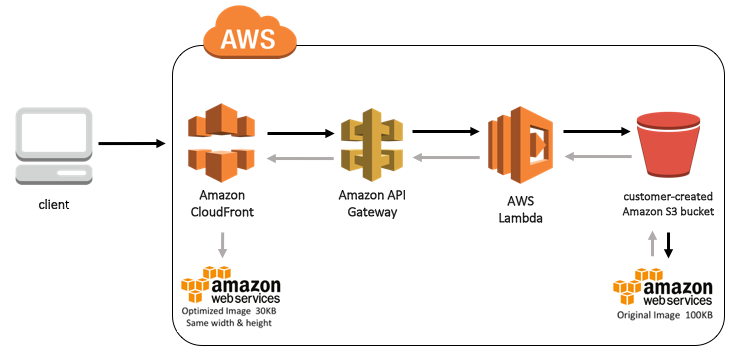
\includegraphics[width=15cm]{serverless-image-handler-architecture}
  \caption[Arquitectura del manejador de imágenes]{Arquitectura del manejador de imágenes. Tomado de \protect\cite{aws-lambda-image-handler}}
  \label{fig:serverless-image-handler-architecture}
\end{figure}

\subsection{\emph{Manejador de imágenes}} \label{sec:manejador-imagenes-1}
Sitios Web con imágenes grandes pueden experimentar tiempos de carga prolongados, es por esto que los desarrolladores proporcionan diferentes versiones de cada imagen para que se acomoden a distintos anchos de banda o diseños de página. Para brindar tiempos de respuesta cortos y disminuir el costo de la optimización, manipulación y procesamiento de las imágenes, AWS propone un manejador de imágenes \emph{serverless}, al cual se le pueda delegar tal trabajo como una función Lambda sobre la plataforma FaaS.


A continuación se describe la arquitectura de la figura \ref{fig:serverless-image-handler-architecture}:
\begin{enumerate}
    \item Amazon CloudFront provee una capa de \emph{cache} para reducir el costo del procesamiento de la imagen
    \item Amazon API Gateway brinda acceso por medio de HTTP a las funciones Lambda
    \item AWS Lambda obtiene la imagen de un repositorio de Amazon Simple Storage Service (Amazon S3) y por medio de la implementación de la función se retorna una versión modificada de la imagen al API Gateway
    \item El API Gateway retorna una nueva imagen a CloudFront para su posterior entrega a los usuarios finales
\end{enumerate}

Cabe mencionar que, en este contexto, una versión modificada de una imagen será cualquier imagen que haya presentado algún tipo de alteración con respeto de una imagen original como, por ejemplo, cambios de tamaño, color, metadatos, etc.

\subsection{Manejador de imágenes para SPE} \label{sec:manejador-imagenes-spe}
Para este estudio se proponemos implementar una variación del manejador de imágenes de la sección \ref{sec:manejador-imagenes-1}, que se muestra en la figura \ref{fig:serverless-image-handler-architecture-spe}.

\begin{figure}[h]
  \centering
  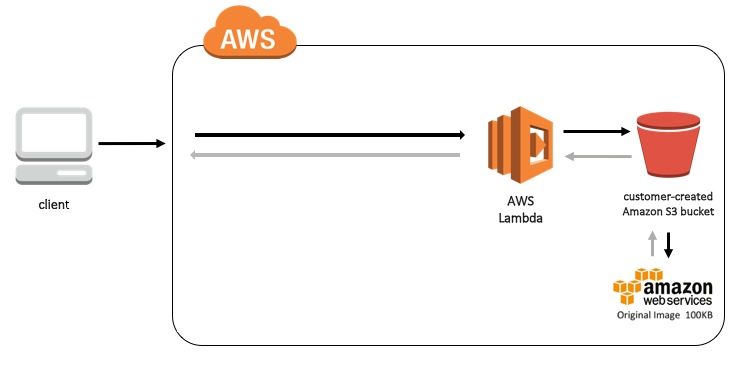
\includegraphics[width=15cm]{serverless-image-handler-architecture-spe}
  \caption[Arquitectura del manejador de imágenes propuesto para el estudio]{Arquitectura del manejador de imágenes propuesto para el estudio.}
  \label{fig:serverless-image-handler-architecture-spe}
\end{figure}

Se han dejado por fuera intencionalmente el AWS CloudFront y el AWS API Gateway. La razón de esto es porque se pretende ejercitar la función Lambda directamente. Se implementará una función Lambda que entregue a partir de una solicitud de redimensionamiento de una imagen almacenada, otra con dimensiones diferentes producida ``al vuelo'' como respuesta a la solicitud. Por ejemplo, si la imagen original mide 500 pixeles de ancho y alto, entregar una con dimensiones de 100 pixeles de ancho y alto. 

Las actividades involucradas en el proceso de redimensionamientos de imágenes se muestran en la figura \ref{fig:serverless-image-handler-architecture-workflow}
\begin{enumerate}
    \item Se envía una solicitud de redimensionamiento de imagen en formato \texttt{JSON} a la función Lambda con los datos acerca de la localización de la imagen y su nuevo tamaño.
    \item La solicitud de redimensionamiento llega a la función Lambda.
    \item La función Lambda solicita al servicio de almacemiento AWS S3 la imagen.
    \item AWS S3 entrega a la función Lambda la imagen solicitada.
    \item La función Lambda inicia el redimensionamiento de la imagen de acuerdo a los parámetros solicitados.
    \item La nueva imagen modificada se entrega al cliente(s).
\end{enumerate}

\begin{figure}[h]
  \centering
  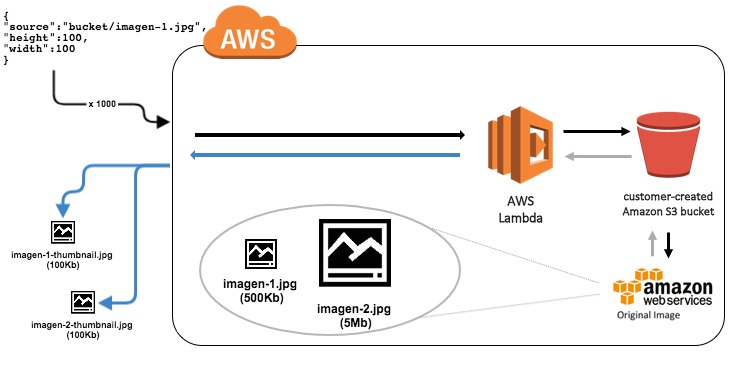
\includegraphics[width=17cm]{serverless-image-handler-architecture-workflow-2}
  \caption[Carga de trabajo sugerida para el manejador de imágenes]{Carga de trabajo sugerida para el manejador de imágenes}
  \label{fig:serverless-image-handler-architecture-workflow}
\end{figure}


A la función Lambda se le realizarán pruebas con imágenes de entrada de distinto tamaño para evaluar su comportamiento bajo estos escenarios, particularmente el tiempo de respuesta de la función. Los resultados obtenidos a partir de estas pruebas van a servir como un punto de referencia para experimentos futuros. La figura \ref{fig:serverless-image-handler-architecture-workflow} muestra una sugerencia de dos posibles cargas de trabajo: 

%\begin{figure}[h]
%  \centering
%  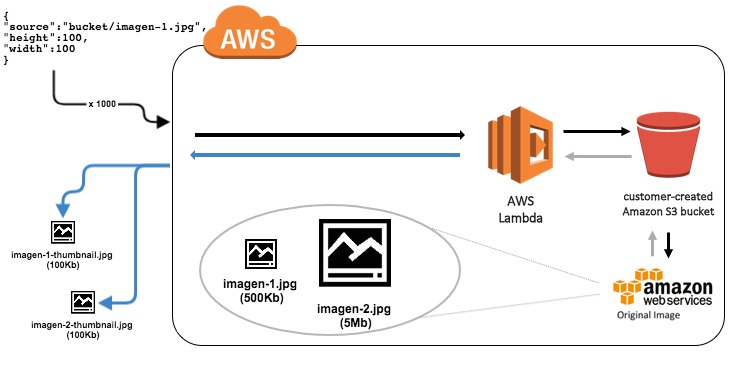
\includegraphics[width=17cm]{serverless-image-handler-architecture-workflow-2}
%  \caption[Carga de trabajo sugerida para el manejador de imágenes]{Carga de trabajo sugerida para el manejador de imágenes}
%  \label{fig:serverless-image-handler-architecture-workflow}
%\end{figure}

\begin{enumerate}
    \item 1000 solicitudes de cambio de tamaño de una imagen grande. En la figura \ref{fig:serverless-image-handler-architecture-workflow}, \texttt{imagen-2.jpg} de tamaño de 5Mb, representa una imagen grande.
    \item 1000 solicitudes de cambio de tamaño de una imagen pequeña. En la figura \ref{fig:serverless-image-handler-architecture-workflow}, \texttt{imagen-1.jpg} de tamaño menor o igual a 500Kb, representa una imagen pequeña.
\end{enumerate}

En principio las cargas de trabajo generadas serían cerradas, lo que quiere decir que una solicitud se ejecuta solamente hasta que la anterior se termina. Esto ayudará en principio a tener mejor trazabilidad de lo que ocurre con la función.

\paragraph{¿Por qué este caso de uso se considera relevante?}
A continuación se listan las características que hacen este caso de uso representativo e interesante:
\begin{itemize}
    \item Sencillo de entender e implementar: se cuenta únicamente con una función la cual lleva a cabo una tarea muy específica.
    \item Popular: sigue un patrón de procesamiento dirigido por eventos y, como se señala en \cite{serverless-architecture-patterns}, este es uno de los más populares que se ha empezado a adoptar para aplicaciones \emph{serverless}. Otra de las razones de la popularidad de este caso de uso es que permite a los desarrolladores crear una unidad de instalación independiente y especializada para el manejo de imágenes, liberando así a sus servidores y aplicaciones del manejo de las peticiones y lógica asociadas a estas.
    \item Replicable en otros proveedores de servicios en la nube: varias de las arquitecturas de referencia para \emph{serverless} propuestas por Amazon, están compuestas por herramientas y servicios muy propios de su plataforma, lo cual hace muy difícil su reproducibilidad utilizando otros proveedores. Aunque en principio este trabajo plantea ser elaborado en la plataforma FaaS de Amazon Web Services, AWS Lambda, otros proveedores de servicios (ver sección \ref{sec:proveedores-faas}) en la nube cuentan con sus propias plataformas de FaaS y de almacenamiento, lo cual permitiría replicar lo aquí propuesto en ellos.
    \item Replicable en los lenguajes de programación soportados por plataformas FaaS: actualmente JavaScript, Java (y lenguajes basados en la \emph{Java Virtual Machine}), Python, C\# y Go son los principales lenguajes de programación soportados por las plataformas FaaS. El caso de uso propuesto, no presenta ningún tipo de característica que lo ate a un lenguaje de programación en particular. En todos ellos se cuentan con bibliotecas para manejo de imágenes tanto de forma nativa como por medio de soluciones de terceros. 
\end{itemize}

\subsection{Experimentos propuestos}

\section{Etapa 2}

\subsection{Modelo de rendimiento a partir de la función}
Las cargas de trabajo descritas en la sección \ref{sec:manejador-imagenes-spe} van a alimentar la bitácora de eventos de la función. En AWS el servicio encargado de llevar registro de los eventos que suceden en una función Lambda se llama Amazon CloudWatch\footnote{\url{https://aws.amazon.com/cloudwatch}}. 

Para obtener un modelo a partir del comportamiento de una función, se propone adoptar un enfoque similar al que se plantea en Walter et al. \cite{Walter:2018:TDP:3185768.3185777}, en donde a partir de lo que los autores llaman un \emph{enfoque de ingeniería de rendimiento declarativo} se logra automatizar gran parte del proceso de ingeniería de rendimiento y también explorar, responder y visualizar aspectos concernientes al rendimiento de un sistema. Esto se alcanza gracias a una serie de herramientas desarrolladas por el grupo de ingeniería de software de la Universidad Würzburg de Alemania y que están disponibles en \url{http://descartes.tools}.

\begin{figure}[h]
  \centering
  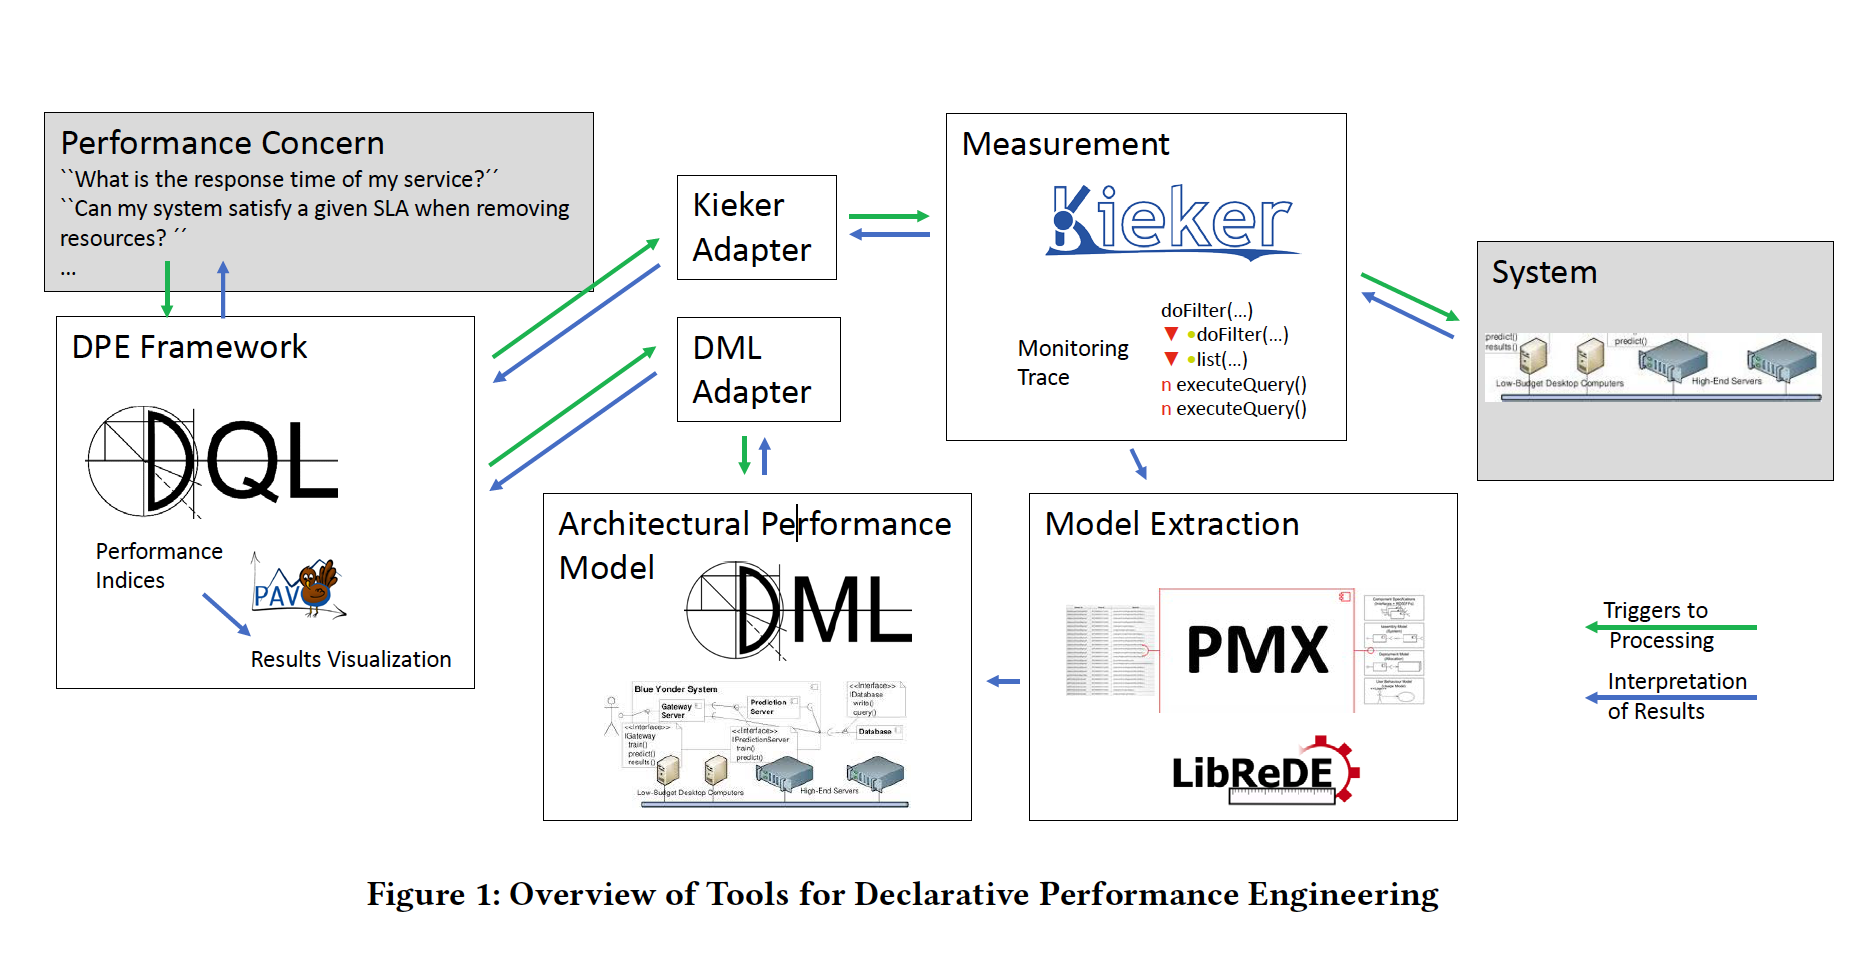
\includegraphics[width=17cm]{declarative-performance-engineering}
  \caption[Herramientas utilizadas para ingeniería de rendimiento declarativo]{Herramientas utilizadas para ingeniería de rendimiento declarativo. Tomado de \cite{Walter:2018:TDP:3185768.3185777}}
  \label{fig:declarative-performance-engineering}
\end{figure}

La figura \ref{fig:declarative-performance-engineering} muestra las herramientas involucradas en el proceso de ingeniería de rendimiento declarativo. Pueden clasificarse en: herramientas para determinar niveles de servicio, para interpretar mediciones obtenidas por medio de la ejecución de un sistema, para extraer modelos de rendimiento y para visualizar resultados. En las figura \ref{fig:declarative-performance-engineering} estas herramientas son:
\begin{itemize}
    \item \textbf{DPE Framework (DPE)}: herramienta para determinar los niveles de servicio de un sistema. Esto lo logra mediante el \emph{Descartes Query Language}(DQL), un lenguaje de consultar indicadores de rendimiento. DPE también incluye \emph{Performance Analysis Visualization} (PAVO) para la visualización de indicadores de rendimiento.
    \item \textbf{Kieker}: una herramienta para el monitoreo del rendimiento de la aplicación (APM por sus siglas en inglés). 
    \item \textbf{Performance Model Extractor (PMX)}: una herramienta que puede derivar modelos de rendimiento a partir de los datos del monitoreo del rendimiento de la aplicación. Puede tomar los datos obtenidos por Kieker y generar modelos de rendimiento en PCM y DML (ver sección \ref{sec:dml})
\end{itemize}

\subsection{Enfoque de trabajo propuesto}
El enfoque que se propone para obtener un modelo de rendimiento a partir de una función, es similar al de Walter et al. \cite{Walter:2018:TDP:3185768.3185777} pero omitimos el uso de las herramientas para determinar y consultar niveles de servicio, y también de visualización. La figura \ref{fig:flujo-de-trabajo-propuesto} muestra los participanes involucrados para lograr esta tarea. 

A partir de las cargas de trabajo a las que fue sometida la función Lambda, métricas de rendimiento serán introducidas dentro del servicio Amazon CloudWatch, este creará la bitácora de la función. Para migrar las métricas de CloudWatch en Kieker, se pretende implementar un adaptador con el fin de tomar una muestra de la bitácora y convertirla a un formato que pueda ser entendido por Kieker. Otra alternativa que se valora es la de publicar las métricas de rendimiento directamente en Kieker  desde la función. 

\begin{figure}[h]
  \centering
  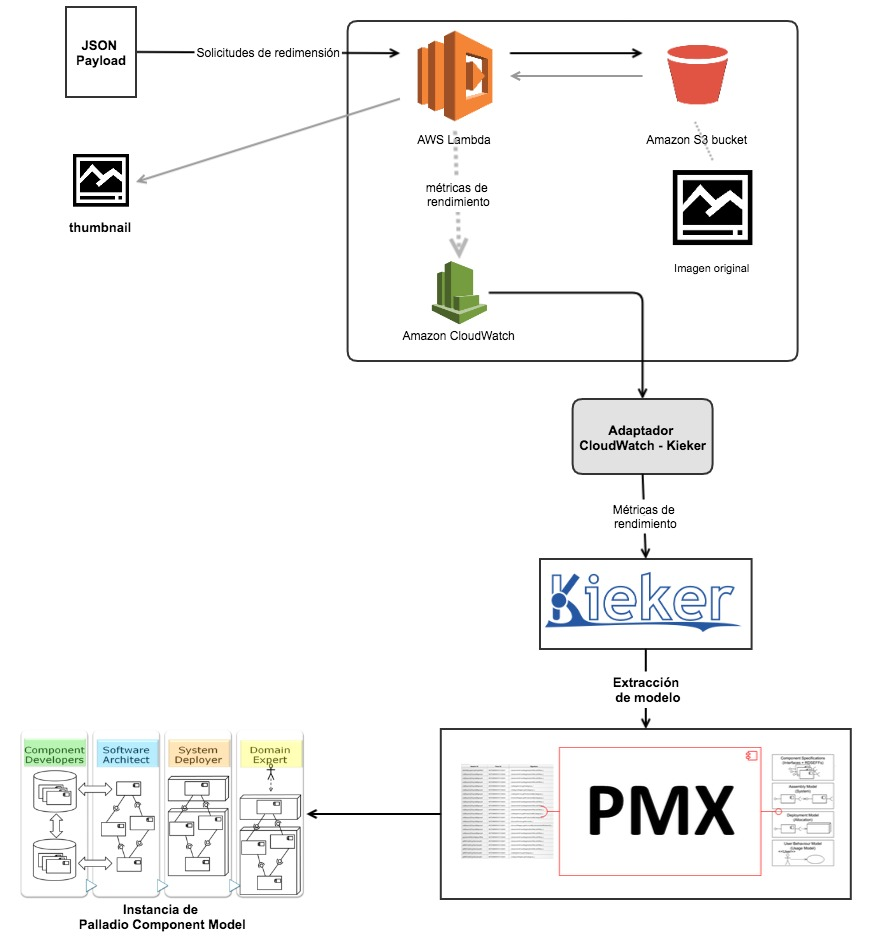
\includegraphics[width=17cm]{flujo-de-trabajo-propuesto-2}
  \caption{Enfoque de trabajo propuesto}
  \label{fig:flujo-de-trabajo-propuesto}
\end{figure}

Una vez que se cuente con una muestra de la ejecución de la función en formato Kieker, esta va a servir como entrada para PMX con el fin de obtener un modelo de rendimiento en PCM. El modelo será utilizado para la ejecución de simulaciones.

\section{Etapa 3: ejecutar simulaciones sobre el modelo obtenido}
\emph{Palladio Workbench}\footnote{\url{https://www.palladio-simulator.com/}} es la herramienta que permite crear y simular modelos basados en PCM. 

Cuando se haya derivado un modelo de rendimiento de la función, se procederá a cargar este modelo en \emph{Palladio Workbench} para modificar y calibrar el modelo y, por medio de las herramientas de simulación que vienen con \emph{Palladio Workbench}, realizar experimentos con el fin de evaluar el grado de coincidencia de los resultados de la simulación con los obtenidos al exponer la función a cargas de trabajo reales.